\documentclass{ncc}
\usepackage[utf8]{inputenc}
\usepackage[russian]{babel}
\usepackage[T2A]{fontenc}
\usepackage{amssymb}
\usepackage{amsmath}
\usepackage{pscyr}
\usepackage{graphicx}
\usepackage{listings}
\usepackage[colorlinks,linkcolor=black,urlcolor=blue]{hyperref}

\lstloadlanguages{C++}
\lstset{
language=C++,
extendedchars=\true, %Чтобы русские буквы в комментариях были
keepspaces=true,
inputencoding=utf8,
breaklines,
columns=fullflexible,
flexiblecolumns,
numbers=left,
numberstyle={\footnotesize},
commentstyle=\it,
stringstyle=\bf,
belowcaptionskip=5pt }


\title{Модель Кронига-Пенни}

\begin{document}
\maketitle

Цель у этого поста одна -- разместить вывод и результаты модели Кронига-Пенни, чтобы больше не тратить на это время. Ну и заодно осмыслить её ещё разок.

В физике твёрдого тела есть проблема, связанная с определением волновых функций электронов в образце. Связана она с тем, что точный учёт взаимодействия электронов делает задачу неразрешимой не только аналитически, но и численно. Что касается численного решения этой задачи, то там есть обходные методы вроде функционала плотности. Качественное же объяснение электронной структуры твёрдых тел можно получить из модели Кронига-Пенни.

От рассмотрения большого количества электронов можно перейти к рассмотрению движения одного электрона в усреднённом потенциале остальных электронов. Из-за периодичности структуры кристаллической решётки логично положить усреднённый потенциал, создаваемый электронами, также периодическим с периодом решётки. Но это не даёт никакой конкретики относительно вида этого потенциала. Самый простейший модельный потенциал, на котором можно ожидать качественно подобного вида спектра, состоит из последовательности прямоугольных потенциальных ям.

\begin{figure}[h!]
    \center
    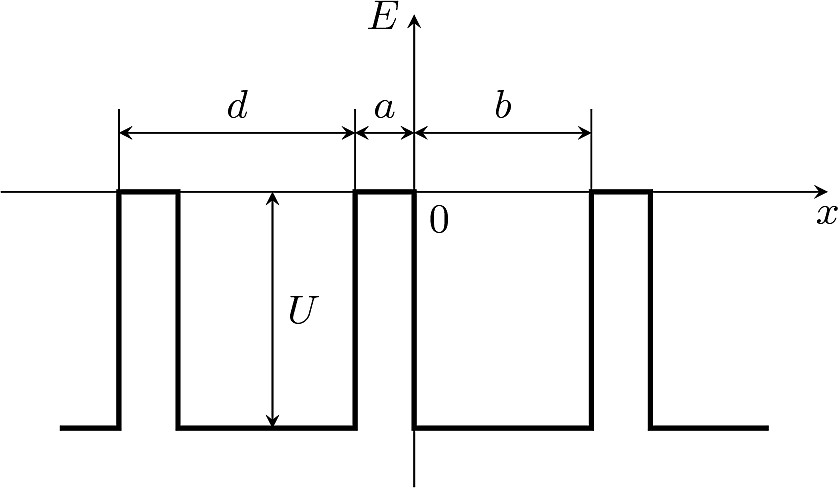
\includegraphics[width=.5\textwidth]{2015-11-09-kronig-penney-potential.png}
    \caption{Потенциал в модели Кронига-Пенни}
\end{figure}

В модели Кронига-Пенни электрон движется в одномерном потенциале, имеющем вид меандра.

Для определения энергии стационарных состояний решим уравнение Шрёдингера в яме и под барьером, а потом сошьём их решение на границе:
\[
  \begin{cases}
    -\frac{\hbar^2}{2m}\Delta \psi_1 = E\psi_1,\
    \left(-\frac{\hbar^2}{2m}\Delta - U\right) \psi_2 = E\psi_2,
  \end{cases}
\]
\[
    \psi_1 = A_1 e^{-i\alpha x} + A_2 e^{i\alpha x},\quad
    \psi_2 = B_1 e^{-i\beta x} + B_2 e^{i\beta x},
\]
где
\[
  \alpha^2 = \frac{2mE}{\hbar^2}, \quad \beta^2 = \frac{2m(E+U)}{\hbar^2}.
\]
Граничные условия на границе первой и второй областей
\[
    \psi_1(0) = \psi_2(0),\quad
    \psi_1^\prime(0) = \psi_2^\prime(0)
\]
Условие на внешних границах этих областей получим из следующих соображений: так как потенциал бесконечен и периодичен, то и наблюдаемые величины должны быть периодичны с тем же периодом. Это означает, что волновая функция на одном периоде потенциала может претерпевать только умножение на некоторый фазовый множитель:
\[
    \psi_1(-a) = e^{ikd}\psi_2(b),\quad
    \psi_1^\prime(-a) = e^{ikd}\psi_2^\prime(b).
\]
Данное обозначение этого множителя имеет свой смысл. Величина \( k \)
называется псевдоволновым вектором электрона и характеризует его перемещение по
решётке вроде того, как волновой вектор характеризует движение свободной частицы
в пространстве.

Запишем эти условия в виде системы уравнений относительно амплитудных коэффициентов:
\[
    \begin{pmatrix}
        1 & 1 & -1 & -1 \
        -i\alpha & i\alpha & i\beta & -i\beta \
        e^{i\alpha a} & e^{-i\alpha a}  & -e^{ikd-i\beta b}  & -e^{ikd+i\beta b} \
        -i\alpha e^{i\alpha a} & i\alpha e^{-i\alpha a}  & i\beta e^{ikd-i\beta b}  &
        -i\beta e^{ikd+i\beta b}
    \end{pmatrix}
    \begin{pmatrix}
        A_1\
        A_2\
        B_1\
        B_2
    \end{pmatrix}
    =
    0
\]
Для существования нетривиального решения необходимо равенство нулю определителя
системы:
\[
    \begin{vmatrix}
        1 & 1 & -1 & -1 \
        -\alpha & \alpha & \beta & -\beta \
        e^{i\alpha a} & e^{-i\alpha a}  & -e^{ikd-i\beta b}  & -e^{ikd+i\beta b} \
        -\alpha e^{i\alpha a} & \alpha e^{-i\alpha a}  & \beta e^{ikd-i\beta b}  &
        -\beta e^{ikd+i\beta b}
    \end{vmatrix}
    =
\]
\[
    =4
    \begin{vmatrix}
        1 & 0 & -1 & 0 \
        -\alpha & \alpha & \beta & -\beta \
    e^{i\alpha a} & -i\sin \alpha a  & -e^{ikd-i\beta b}  & -ie^{ikd}\sin\beta b \
        -\alpha e^{i\alpha a} & \alpha \cos\alpha a & \beta e^{ikd-i\beta b}  &
        -\beta e^{ikd}\cos\beta b
    \end{vmatrix}
    =
\]
\[
    =4
    \begin{vmatrix}
        1 & 0 & 1 & 0 \
        0 & \alpha & 0 & \beta \
    \cos\alpha a & -i\sin \alpha a  & e^{ikd}\cos \beta b  & ie^{ikd}\sin\beta b \
        -i\alpha \sin\alpha a & \alpha \cos\alpha a & i \beta e^{ikd} \sin{\beta b}  &
        \beta e^{ikd}\cos\beta b
    \end{vmatrix}
    =
\]
\[
    =4
    \begin{vmatrix}
        1 & 0 & 0 & 0 \
        0 & \alpha & 0 & \beta \
    \cos\alpha a & -i\sin \alpha a  & e^{ikd}\cos \beta b - \cos\alpha a  & ie^{ikd}\sin\beta b \
        -i\alpha \sin\alpha a & \alpha \cos\alpha a & i \beta e^{ikd} \sin{\beta
    b} + i\alpha\sin\alpha a  &
        \beta e^{ikd}\cos\beta b
    \end{vmatrix}
    =
\]
\[
    =4\alpha\beta
    \begin{vmatrix}
        1 & 0 & 1 \
        -\frac{i}{\alpha}\sin \alpha a  & e^{ikd}\cos \beta b - \cos\alpha a  &
        \frac{i}{\beta} e^{ikd}\sin\beta b \
        \cos\alpha a & i\beta e^{ikd} \sin{\beta
    b} + i\alpha\sin\alpha a  &
        e^{ikd}\cos\beta b
    \end{vmatrix}
    =
\]
\[
    =4\alpha\beta
    \begin{vmatrix}
        1 & 0 & 0 \
        -\frac{i}{\alpha}\sin \alpha a  & e^{ikd}\cos \beta b - \cos\alpha a  &
        \frac{i}{\beta} e^{ikd}\sin\beta b + \frac{i}{\alpha}\sin \alpha a  \
        \cos\alpha a & i\beta e^{ikd} \sin{\beta
    b} + i\alpha\sin\alpha a  &
        e^{ikd}\cos\beta b-\cos\alpha a
    \end{vmatrix}
    =
\]
\[
    =4\alpha\beta
    \begin{vmatrix}
        e^{ikd}\cos \beta b - \cos\alpha a  &
        \frac{i}{\beta} e^{ikd}\sin\beta b + \frac{i}{\alpha}\sin \alpha a  \
        i\beta e^{ikd} \sin{\beta b} + i\alpha\sin\alpha a  &
        e^{ikd}\cos\beta b-\cos\alpha a
    \end{vmatrix} = 0
\]
Раскрывая этот простейший определитель, получаем:
\[
    (e^{ikd}\cos \beta b - \cos\alpha a) (e^{ikd}\cos\beta b -
    \cos\alpha a) +
\]
\[
    + \frac{1}{\alpha\beta}(\beta e^{ikd} \sin{\beta b} + \alpha\sin\alpha a)(\alpha
    e^{ikd}\sin\beta b + \beta \sin\alpha a) = 0,
\]
\[
    e^{2ikd} - (2\cos\alpha a \cos\beta b -
    \frac{\alpha^2 + \beta^2}{\alpha\beta}\sin\alpha a \sin\beta b)e^{ikd} +
    1 = 0,
\]
\[
    \cos kd = \cos\alpha a\cos\beta b - \frac{\alpha^2
    +\beta^2}{2\alpha\beta}\sin\alpha a \sin\beta b.
\]

Уже из вида этого дисперсионного соотношения можно сделать выводы относительно
характера спектра. Так как для периодических решений \( k \in \mathbb{R} \),
то \( |\cos kd| \le 1 \). Это условие может выполняться не для всех значений
энергии. Полосы, в которых оно выполняется являются разрешёнными зонами, а те, в
которых не выполняется -- запрещёнными.

Не прибегая пока к численному решению, рассмотрим некоторые предельные случаи:
\begin{itemize}
  \item \( U = 0,\ \alpha=\beta \) -- свободная частица: \[ \cos kd = \cos\alpha
    d,\ k = \alpha,\ E = \frac{\hbar^2 k^2}{2m}; \]
  \item \( Ub = \mathrm{const},\ b\to0 \) -- потенциал в форме гребёнки Дирака
    \[
        \cos kd = \cos\alpha a - \frac{\beta^2 b}{2\alpha}\sin\alpha a.
    \]
\end{itemize}
Ну а теперь результаты расчётов. При \( a = 0{,}5~nm,\) \( b = 0{,}1~nm,\)
\(U=10~eV \) получается следующая картина:
\begin{figure}[h!]
\center
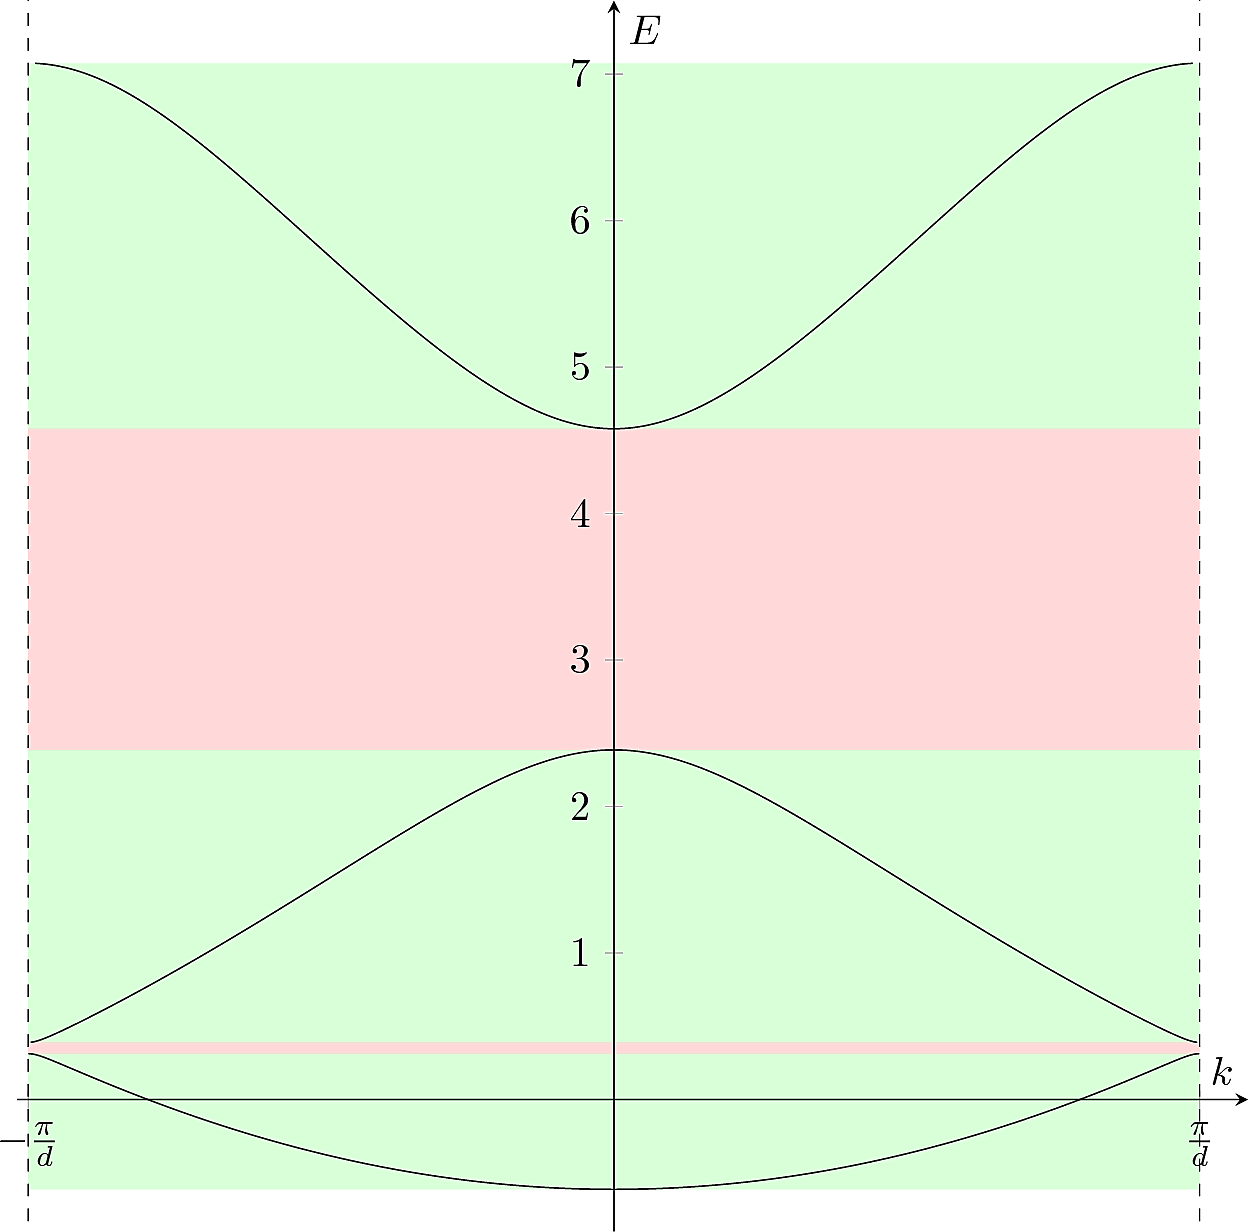
\includegraphics[width=.5\textwidth]{2015-11-09-kronig-penney-bands.png}
\end{figure}

Здесь зелёным подкрашены разрешённые зоны, а красным -- запрещённые. Таким образом, даже очень упрощённая модель может обладать основными свойствами
очень сложной системы.
\end{document}
